\section{大数定律与中心极限定理}
    
    \frame{\sectionpage}
    
     \begin{frame}{特征函数和概率极限定理}
    \begin{itemize}
    	\item 随机变量的收敛性
    	
    	$\quad$依分布收敛、依概率收敛、几乎处处收敛、$L^p$收敛
    	\item 概率母函数、特征函数
    	\item 大数定律
    	\item 中心极限定理
    \end{itemize}
\end{frame}

\begin{frame}{\textbf{概率母函数} Probability Generating Function}
		\begin{block}{\textbf{Def 1.1}$\quad$对一个只取非负整数值的离散型随机变量$X$}
		其母函数定义为\begin{equation}
			g(s) = \mathrm{E}(s^X) = \sum_{j=0}^\infty s^jP(X=j),s\in [-1,1].
		\end{equation}
	\end{block}
	概率母函数的引入为计算取非负整数值的随机变量的概率分布、数学期望和方差等带来了很多的方便.
	\begin{itemize}
		\item 这个定义的存在性是由于$|s^X|\leqslant 1$保证了所求数学期望的存在性;
		\item 此处约定$0^0 = 1$.
	\end{itemize}

\end{frame}

\begin{frame}{\textbf{概率母函数} Probability Generating Function}
\begin{block}{\textbf{Thm 1.1}假设$g(s)$是$X$的母函数,则有}
	\begin{itemize}
		\item $P(X=k) = \frac{1}{k!}g^{(k)}(0),k=0,1,\cdots$;
		\item $\mathrm{E}X = g'(1)$;
		\item 如果$\mathrm{E}X<\infty$,则$\mathrm{var}(X) = g''(1)+g'(1)-(g'(1))^2$;
		\item 如果$X_1,X_2,\cdots,X_n$相互独立,$g_j(s) = \mathrm{E}s^{X_j}$是$X_j$的母函数,则$Y = X_1+X_2+\cdots+X_n$有母函数
		\begin{equation}
			g_Y(s) = g_1(s)g_2(s)\cdots g_n(s),s\in [-1,1].
		\end{equation}
	\end{itemize}	
\end{block}
\end{frame}

\begin{frame}
	\textbf{证明}$\quad$
	
	(1)\begin{equation}
		\begin{split}
			\frac{1}{k!}g^{(k)}(0) &= \frac{1}{k!}g^{(k)}(s)\bigg|_{s=0} \\
			&= \frac{1}{k!}\sum_{j=k}^\infty\frac{\mathrm{d}^k}{\mathrm{d}s^k}(s^j)P(X=j)\bigg|_{s=0} \\
			&= P(X=k).
		\end{split}
	\end{equation}
	
	(2)由$g'(1) = \sum\limits_{j=0}^\infty jP(X=j) = \mathrm{E}X$得到.
	
	(3)由\begin{equation}
		g''(1) = \sum_{j=0}^\infty j(j-1)P(X=j) = \mathrm{E}[X(X-1)]
	\end{equation}
\end{frame}

\begin{frame}
	得到\begin{equation}
		g''(1)+g'(1) - (g'(1))^2 = \mathrm{E}[X(X-1)] + \mathrm{E}X - (\mathrm{E}X)^2 = \mathrm{var}(X).
	\end{equation}
	
	(4)由于$X_1,X_2,\cdots,X_n$相互独立,所以随机变量$s^{X_1},s^{X_2},\cdots,s^{X_n}$相互独立.
	
	又由于$\left|s^{X_1+X_2+\cdots+X_n}\right|\leqslant 1$,所以可以使用Fubini定理,因此,
	\begin{equation}
		g_Y(s) = \mathrm{E}s^{X_1+X_2+\cdots+X_n} = \mathrm{E}s^{X_1}\cdots\mathrm{E}s^{X_n} = g_1(s)g_2(s)\cdots g_n(s)
	\end{equation}
	
	Rmk:结论(1)说明了对于只取非负整数值的随机变量,\alert{母函数和概率分布相互唯一决定}(determine).
\end{frame}

\begin{frame}
	\textbf{例}$\quad$二项分布$\mathcal{B}(n,p)$的母函数是
	\begin{equation}
		g(s) = \sum_{j=0}^ns^j\binom{n}{j}p^jq^{n-j} = (q+sp)^n.
	\end{equation}
	此外,设$X_1,X_2,\cdots,X_m$相互独立,$X_j\sim \mathcal{B}(n_j,p)$,则
	\begin{equation}
		Y = X_1+X_2+\cdots+X_m
	\end{equation}
	有母函数
	\begin{equation}
		\begin{split}
			g_Y(s) &= (q+sp)^{n_1}\cdots(q+sp)^{n_m} \\
			&= (q+sp)^n,n = n_1+\cdots+n_m.
		\end{split}
	\end{equation}
	说明$Y\sim\mathcal{B}(n_1+\cdots+n_m,p)$.
\end{frame}

\begin{frame}
	\textbf{例}$\quad$泊松分布$\mathcal{P}(\lambda)$的母函数是
	\begin{equation}
		g(s) = \sum_{k=0}^\infty s^k\frac{\lambda^k}{k!}e^{-\lambda} = e^{\lambda (s-1)}.
	\end{equation}
	此外,设$X_1,X_2,\cdots,X_m$相互独立,$X_j\sim \mathcal{P}(\lambda_j)$,则
	\begin{equation}
	Y = X_1+X_2+\cdots+X_m
	\end{equation}
	有母函数
	\begin{equation}
	\begin{split}
	g_Y(s) &= e^{\lambda_1 (s-1)}\cdots e^{\lambda_m (s-1)} \\
	&= e^{\lambda (s-1)},\lambda = \lambda_1+\cdots+\lambda_m.
	\end{split}
	\end{equation}
	说明$Y\sim\mathcal{P}(\lambda_1+\cdots+\lambda_m)$.
\end{frame}

\begin{frame}
	\textbf{例}$\quad$$X$服从几何分布$\mathcal{G}(p)$,它有母函数\begin{equation}
		g(s) = \sum_{j=1}^\infty s^jpq^{j-1} = \frac{sp}{1-sq}.
	\end{equation}
	此外,设$X_1,X_2,\cdots,X_m$相互独立,都服从相同的几何分布$\mathcal{G}(p)$,则
	$Y = X_1+X_2+\cdots+X_m$有母函数
	\begin{equation}
		g_Y(s) = \left(\frac{sp}{1-sq}\right)^m.
	\end{equation}
	将上式的右边进行Taylor展开,得到
	\begin{equation}
	\begin{split}
		g_Y(s) &= (sp)^m\sum_{j=0}^\infty \frac{m(m+1)\cdots(m+j-1)}{j!}(sq)^j \\
		&= (sp)^m\sum_{j=0}^\infty\binom{m+j-1}{m-1}(sq)^j \\
		&= \sum_{k=m}^\infty\binom{k-1}{m-1}p^mq^{k-m}s^k
	\end{split}
	\end{equation}
\end{frame}

\begin{frame}
	于是得到Pascal(帕斯卡)分布
	\begin{equation}
		P(Y=k) = \binom{k-1}{m-1}p^mq^{k-m},k=m,m+1,\cdots.
	\end{equation}
	回忆在前面的讨论中,$Y$是第$m$次击中目标时的射击总次数.
	\\ \hspace*{\fill} \\%空行
	\textbf{练习}$\quad$掷三枚骰子,求点数之和是9的概率.
	
	\textbf{解}$\quad$用$X_i$表示第$i$颗骰子的点数,$i=1,2,3$,则$Y=X_1+X_2+X_3$是三颗骰子的总点数.由
	\begin{equation}
		g(s) = \mathrm{E}s^{X_1} = \frac{1}{6}(s+s^2+\cdots+s^6) = \frac{1}{6}\frac{s(1-s^6)}{1-s}.
	\end{equation}
\end{frame}

\begin{frame}
	得到$Y$的母函数\begin{equation}
	\begin{split}
		g_Y(s) &= g^3(s) = \frac{s^3(1-s^6)^3}{6^3(1-s)^3} \\
		&= \frac{1}{6^3}s^3(1-3s^6+3s^{12}-s^{18})\sum_{k=0}^\infty\binom{k+2}{2}s^k.
	\end{split}
	\end{equation}
	可以算出$s^9$的系数是
	\begin{equation}
		P(Y=9) = \frac{1}{6^3}\left(\binom{6+2}{2}-3 \right) = \frac{25}{216}.
	\end{equation}
	\textbf{练习}$\quad$设$p=1-q\in(0,1)$,验证对数正态分布\begin{equation}
		P(X=k) = -\frac{q^k}{k\ln p},k=1,2,\cdots
	\end{equation}
	的母函数和数学期望分别是\begin{equation}
		\frac{\ln(1-qs)}{\ln p}\text{和}\frac{-q}{p\ln p}.
	\end{equation}
\end{frame}

\begin{frame}{\textbf{特征函数} Characteristic Function}
\begin{block}{\textbf{Def 2.1}如果$\xi,\eta$是随机变量,$i=\sqrt{-1}$,则称}
	\begin{equation}
		Z=\xi + i\eta
	\end{equation}
	是复值随机变量.如果$\mathrm{E}\xi,\mathrm{E}\eta$都存在,则$Z$的数学期望为
	\begin{equation}
		\mathrm{E}Z = \mathrm{E}\xi + i\mathrm{E}\eta.
	\end{equation}
\end{block}
没有特殊声明时,以下讨论的随机变量还都是实值的.
\end{frame}

\begin{frame}{\textbf{特征函数} Characteristic Function}
\begin{block}{\textbf{Def 2.2}对随机变量$X$,}
	由于$\sin(tX),\cos(tX)$的数学期望都存在,于是可以定义\begin{equation}
	\phi(t) \stackrel{\text{def}}{=}\mathrm{E}e^{itX} = \mathrm{E}\cos(tX) + i\mathrm{E}\sin(tX),t\in\mathbb{R}
	\end{equation}
	称上式定义的$\phi(t)$为$X$的\alert{特征函数}.
\end{block}
\begin{itemize}
	\item 当$X$为离散型时: $P(X=x_k) = p_k,k=1,2,\cdots$,
	\begin{equation}
		\phi(t) = \sum_{k}e^{itx_k}p_k.
	\end{equation}
	\item 当$X$为连续型时:$X$有密度$f(x)$
	\begin{equation}
		\phi(t) = \int_{-\infty }^\infty e^{itx}f(x)\mathrm{d}x.
	\end{equation}
\end{itemize}
\end{frame}

\begin{frame}
	\textbf{Rmk1}:不同的数学群体对于\alert{Fourier变换}的定义会略有不同.
	\begin{itemize}
		\item 不少的文献把$F$的Fourier-Stieltjes变换定义成
			\begin{equation}
				\frac{1}{(2\pi)^n}\int_{\mathbb{R}^n}\exp(-i\bm{\xi}\cdot\bm{y})\mathrm{d}F(\bm{y}).
			\end{equation}
		\item 有些文献则把$F$的Fourier-Stieltjes变换定义成
			\begin{equation}
				\int_{\mathbb{R}^n}\exp(i\bm{t}\cdot\bm{y})\mathrm{d}F(\bm{y}).
			\end{equation}
	\end{itemize}
	概率论的文献中通常使用后一个定义,且把Fourier变换改称为\textbf{特征函数}.这样的差异仅仅是Fourier变换及逆变换的公式的形式上的,并不会给数学理论带来重大的改变.
	
	\textbf{Rmk2}:在概率论以外的其它的数学分支中,还有一些不同含义的函数也被称为"特征函数",切勿与此混淆,一个是线性算子的特征函数(本征函数),另一个是集合的特征函数(指示函数、示性函数)
\end{frame}

\begin{frame}
	\textbf{Rmk3}:对每个分布函数$F$,可以在$\mathbb{R}$上引进唯一的一个Borel测度$\mu$,使得任何满足条件的$a\leqslant b$的实数$a$和$b$,都有以下等式:
	\begin{equation}
		\mu((a,b]) = F(b) - F(a).
	\end{equation}
	这个Borel测度$\mu$时常记作$\mu = \mathrm{d}F$.
	
	特征函数也常记作\begin{equation}
		\phi(t) = \int_{-\infty}^\infty e^{itx}\mu(\mathrm{d}x).
	\end{equation}
	多元的情况也有类似的公式.
\end{frame}

\begin{frame}
	\textbf{例}$\quad$(Coin Flips)设$P(X=1) = P(X=-1) = 1/2$,则
	\begin{equation}
		\mathrm{E}e^{itX} = (e^{it}+e^{-it})/2 = \cos t.
	\end{equation}
	
	\textbf{例}$\quad$(Poisson分布)设$P(X=k) = e^{-\lambda}\lambda^k/k!$,for $k = 0,1,2,\cdots$
	\begin{equation}
		\mathrm{E}e^{itX} = \sum_{k=0}^\infty e^{-\lambda}\frac{\lambda^k e^{itk}}{k!} = \exp(\lambda (e^{it}-1)).
	\end{equation}
	
	\textbf{例}$\quad$(二项(Binomial)分布)设$X\sim \mathcal{B}(n,p)$
	\begin{equation}
	\begin{split}
		\mathrm{E}e^{itX} &= \sum_{k=0}^n\binom{n}{k}p^kq^{n-k}e^{itk} \\
		&=\sum_{k=0}^n\binom{n}{k}(pe^{it})^kq^{n-k} \\
		&=(pe^{it}+q)^n.
		\end{split}
	\end{equation}
	
\end{frame}

\begin{frame}
	\textbf{例}$\quad$(几何分布)设$X\sim\mathcal{G}(p),P(X=k)=pq^{k-1},k=1,2,\cdots.$
	\begin{equation}
	\begin{split}
	\mathrm{E}e^{itX} &= \sum_{k=1}^\infty pq^{k-1}e^{itk} \\
	&=\sum_{k=1}^\infty pe^{it}(qe^{it})^{k-1}\\
	&=\frac{pe^{it}}{1-qe^{it}}.
	\end{split}
	\end{equation}
	
	\textbf{例}$\quad$(负二项分布)设$P(X=k)=\binom{k+r-1}{r-1}q^kp^r,k=0,1,\cdots$,其中$p+q=1,pq>0.$
	\begin{equation}
	\begin{split}
	\mathrm{E}e^{itX} &= \sum_{k=0}^\infty \binom{k+r-1}{r-1}q^kp^re^{itk} \\
	&=\left(\frac{p}{1-qe^{it}}\right)^r.
	\end{split}
	\end{equation}
\end{frame}


\begin{frame}
	\textbf{例}$\quad$Uniform distribution on $(a,b)$
	
	解: 根据
	\begin{equation}
		\int_{a}^{b}e^{\lambda x}\mathrm{d}x = (e^{\lambda b}-e^{\lambda a})/\lambda,\forall \lambda\in\mathbb{C}
	\end{equation}	
	得到
	\begin{equation}
	\begin{split}
	\phi(t) &= \int_{-\infty}^\infty e^{itx}f(x)\mathrm{d}x \\
	&=\int_{a}^b e^{itx}/(b-a)\mathrm{d}x  \\
	&= \frac{e^{itb}-e^{ita}}{it(b-a)}.
	\end{split}
	\end{equation}
	Special Case:$(a,b)=(-c,c)$,
	
	Ch.f. $\phi(t) = \frac{\sin(ct)}{ct}$.
	
\end{frame}

\begin{frame}
	\textbf{例}$\quad$(Exponential distribution)设$X\sim\mathcal{E}(\lambda)$.
	
	Density:\begin{equation}
		f(x) =\lambda e^{-\lambda x}\bm{1}_{(x>0)}.
	\end{equation}

	Ch.f.:\begin{equation}
		\phi(t) = \int_{0}^\infty e^{itx}\lambda e^{-\lambda x}\mathrm{d}x = \frac{\lambda e^{(it-\lambda)x}}{it-\lambda}\bigg|^{+\infty}_0 = \frac{\lambda}{\lambda - it}.
	\end{equation}
	since:$|e^{(it-\lambda)x}| = e^{-\lambda x}\to 0$, as $x\to+\infty$

\end{frame}

\begin{frame}
\textbf{例}$\quad$(标准正态分布)设$X\sim\mathcal{N}(0,1)$.

Ch.f.:\begin{equation}
\phi(t) = \int_{\mathbb{R}}e^{itx}\frac{1}{\sqrt{2\pi}}e^{-x^2/2}\mathrm{d}x.
\end{equation}
形式上的计算(cheat):
\begin{equation}
	\int_{\mathbb{R}}e^{itx}\frac{1}{\sqrt{2\pi}}e^{-x^2/2}\mathrm{d}x = 
	e^{-t^2/2}\int_{\mathbb{R}}\frac{1}{\sqrt{2\pi}}e^{-(x-it)^2/2}\mathrm{d}x = e^{-t^2/2}.
\end{equation}
数学上的证明:
\begin{equation}
	\begin{split}
		\phi(t) &= \int_{\mathbb{R}}e^{itx}\frac{1}{\sqrt{2\pi}}e^{-x^2/2}\mathrm{d}x\\
		&= \int_{\mathbb{R}}\cos(tx)\frac{1}{\sqrt{2\pi}}e^{-x^2/2}\mathrm{d}x.
	\end{split}
\end{equation}
since: $\sin(tx)$:odd.
\end{frame}

\begin{frame}
	\begin{equation}
	\begin{split}
	\phi'(t) &= \int_{\mathbb{R}}-x\sin(tx)\frac{1}{\sqrt{2\pi}}e^{-x^2/2}\mathrm{d}x\\
	&= -\int_{\mathbb{R}}t\cos(tx)\frac{1}{\sqrt{2\pi}}e^{-x^2/2}\mathrm{d}x\text{(分部积分)}\\
	&= -t\phi(t)
	\end{split}
	\end{equation}
	\begin{equation*}
		\phi'(t) = -t\phi(t)\xRightarrow[]{implies} \frac{\mathrm{d}}{\mathrm{d}t}\{\phi(t)\exp(t^2/2)\} = 0.
	\end{equation*}
	因此,$\phi(t)\exp(t^2/2) = \phi(0) = 1.$证毕.
	评:此例中用到了著名的\textbf{Fresnel积分},这两个积分是Fresnel在研究光学中首次碰到的.
\end{frame}

\begin{frame}
	\textbf{例}$\quad$($\Gamma(\alpha,\beta)$分布)设$X$有密度
	\begin{equation}
		f(x) = \frac{\beta^\alpha}{\Gamma(\alpha)}x^{\alpha-1}e^{-\beta x}\bm{1}_{(x>0)}.
	\end{equation}
	则特征函数为:
	\begin{equation}
		\begin{split}
			\phi(t) &= \int_{0}^\infty  \frac{\beta^\alpha}{\Gamma(\alpha)}x^{\alpha-1}e^{-\beta x}e^{itx}\mathrm{d}x \\
			&=  \frac{\beta^\alpha}{(\beta-it)^\alpha \Gamma(\alpha)}\int_{0}^\infty ((\beta-it)x)^\alpha e^{(it-\beta)x}\frac{\mathrm{d}x}{x} \\
			&= \frac{\beta^\alpha}{(\beta-it)^\alpha}.(\text{形式上})
		\end{split}
	\end{equation}
	Rmk:数学上可以通过复变函数的相关知识对上式进行严格的证明(略).
\end{frame}


\begin{frame}{\textbf{特征函数} Characteristic Function}
	特征函数的最重要的性质之一是如下的逆转公式(下面的证明不要求)
	\begin{block}{\textbf{Thm 2.1}(逆转公式)设$\phi(t)$是$X$的特征函数,$F(x)$是$X$的分布函数,则}
		\begin{equation}
			\overline{F}(b)-\overline{F}(a) = \frac{1}{2\pi}\lim_{T\to\infty}\int_{-T}^{T}\frac{e^{-itb}-e^{-ita}}{-it}\phi(t)\mathrm{d}t.
		\end{equation}
		\begin{itemize}
			\item 其中$\overline{F}(x) = \frac{F(x^+)+F(x^-)}{2},\forall x\in \mathbb{R}$
			\item $t=0$时,$\frac{e^{-itb}-e^{-ita}}{-it}$定义成$b-a$.
		\end{itemize}
	\end{block}
\end{frame}

\begin{frame}
	证明: 不妨设$a<b$,由于\begin{equation}
		\begin{split}
			\left|\frac{e^{-itb}-e^{-ita}}{-it} \right| &= \left|\int_{a}^{b}e^{-itx}\mathrm{d}x\right| \\
			 &\leqslant \int_{a}^{b}\left|e^{-itx}\right|\mathrm{d}x = b-a.
		\end{split}
		\end{equation}
		所以可以应用Fubini定理得到:
		\begin{equation}
		\begin{split}
			I_T &\stackrel{\text{def}}{=}\frac{1}{2\pi}\int_{-T}^{T}\frac{e^{-itb}-e^{-ita}}{-it}\phi(t)\mathrm{d}t \\
			&= \frac{1}{2\pi}\int_{-T}^{T}\frac{e^{-itb}-e^{-ita}}{-it}\int_{\mathbb{R}}e^{itx}\mathrm{d}F(x)\mathrm{d}t \\
			&=\frac{1}{2\pi}\int_{\mathbb{R}}\int_{-T}^{T}\frac{e^{it(x-b)}-e^{it(x-a)}}{-it}\mathrm{d}t\mathrm{d}F(x)
		\end{split}
		\end{equation}
\end{frame}

\begin{frame}
	根据奇偶性,将上式化简为
	\begin{equation}
		I_T=\frac{1}{\pi}\int_{\mathbb{R}}\int_{0}^{T}\frac{\sin(t(x-b))-\sin(t(x-a))}{-t}\mathrm{d}t\mathrm{d}F(x)
	\end{equation}
	记\begin{equation}
		J_T=\int_{0}^{T}\frac{\sin(t(x-b))-\sin(t(x-a))}{-t}\mathrm{d}t.
	\end{equation}
	根据\begin{equation}
		\int_{0}^{T}\frac{\sin(\alpha t)}{t}\mathrm{d}t = \int_{t=0}^{T}\frac{\sin(\alpha t)}{\alpha t}\mathrm{d}(\alpha t).
	\end{equation}
	回忆数学分析的结论:
	\begin{equation}
		\lim_{T\to\infty}\int_{0}^T\frac{\sin t}{t}\mathrm{d}t = \frac{\pi}{2}.
	\end{equation}
\end{frame}

\begin{frame}
	由此便得到:\begin{equation}
		\lim_{T\to\infty}J_T = 	\left\{
		\begin{aligned}
		&0, x<a\ or\ x>b \\
		&\frac{\pi}{2},x=a\ or\ x=b \\
		&\pi, a<x<b
		\end{aligned}
		\right.
	\end{equation}
	即\begin{equation}
		\lim_{T\to\infty}J_T = \frac{\pi}{2}[\bm{1}_{(a\leqslant x<b)}+\bm{1}_{(a<x\leqslant b)}].
	\end{equation}
	由Lebesgue有界收敛定理,\begin{equation}
	\begin{split}
		\lim_{T\to\infty}I_T &= \frac{1}{\pi}\int_{\mathbb{R}}\lim_{T\to\infty}J_T\mathrm{d}F(x) \\
		&= \frac{1}{\pi}\int_{\mathbb{R}}\frac{\pi}{2}[\bm{1}_{(a\leqslant x<b)}+\bm{1}_{(a<x\leqslant b)}]\mathrm{d}F(x) \\
		&= \frac{1}{2}[F(b^-)-F(a^-)]+\frac{1}{2}[F(b)-F(a)] \\
		&= \overline{F}(b)-\overline{F}(a).
	\end{split}		
	\end{equation}
	证毕.
\end{frame}

\begin{frame}
	\textbf{Rmk1}:这个定理也可以写作:
	\begin{equation}
	\mu((a,b)) + \frac{1}{2}\mu(\{a,b\}) = \frac{1}{2\pi}\lim_{T\to\infty}\int_{-T}^{T}\frac{e^{-itb}-e^{-ita}}{-it}\phi(t)\mathrm{d}t.
	\end{equation}
	
	\textbf{Rmk2}:若$a$和$b$是分布函数$F(x)$的连续点,我们便得到
	\begin{equation}
	F(b)-F(a) = \frac{1}{2\pi}\lim_{T\to\infty}\int_{-T}^{T}\frac{e^{-itb}-e^{-ita}}{-it}\phi(t)\mathrm{d}t.
	\end{equation}
\end{frame}

\begin{frame}
\begin{block}{\textbf{Thm $2.1^*$}(逆转公式)设$\phi(t)$是$X$的特征函数,$F(x)$是$X$的分布函数,则}
	如果\begin{equation}
	\int_{-\infty}^\infty |\phi(t)|\mathrm{d}t<\infty
	\end{equation},
	则$X$还有有界且连续的概率密度函数$f(x)$,使得累积概率测度分布函数$F(x)$可以表示成
	\begin{equation}
	F(x) = \int_{-\infty}^x f(y)\mathrm{d}y.
	\end{equation}
	进一步,概率密度$f(x)$可以通过特征函数$\phi(t)$用以下的反演公式表示:
	\begin{equation}
	f(x) = \frac{1}{2\pi}\int_{-\infty}^\infty e^{-itx}\phi(t)\mathrm{d}t.
	\end{equation}
\end{block}
\end{frame}

\begin{frame}
	证明:由于\begin{equation}
		\left|\frac{e^{-itb}-e^{-ita}}{-it} \right|\leqslant |b-a|.
	\end{equation}
	所以得到:
	\begin{equation}
		\begin{split}
			\mu((a,b)) + \frac{1}{2}\mu(\{a,b\}) &= \frac{1}{2\pi}\lim_{T\to\infty}\int_{-T}^{T}\frac{e^{-itb}-e^{-ita}}{-it}\phi(t)\mathrm{d}t \\
			&\leqslant \frac{b-a}{2\pi}\lim_{T\to\infty}\int_{-T}^{T}|\phi(t)|\mathrm{d}t
		\end{split}
	\end{equation}
	这说明$\mu$没有点测度.进一步,运用Fubini-Tonelli定理知道:
	\begin{equation}
		\begin{split}
			\mu((x,x+h)) &= \frac{1}{2\pi}\lim_{T\to\infty}\int_{-T}^{T}\frac{e^{-it(x+h)}-e^{-itx}}{-it}\phi(t)\mathrm{d}t \\
			&= \frac{1}{2\pi}\int_{-\infty}^{\infty}\left(\int_{x}^{x+h}e^{-ity}\mathrm{d}y\right)\phi(t)\mathrm{d}t \\
			&= \lim_{T\to\infty} \int_{x}^{x+h}\left(\frac{1}{2\pi}\int_{-\infty}^{\infty}e^{-ity}\phi(t)\mathrm{d}t \right)\mathrm{d}y
		\end{split}
	\end{equation}
\end{frame}

\begin{frame}
	这说明,$\mu$有密度函数\begin{equation}
		f(y) = \frac{1}{2\pi}\int_{-\infty}^{\infty}e^{-ity}\phi(t)\mathrm{d}t
	\end{equation}
	再根据控制收敛定理知道$f(x)$连续.
	\\ \hspace*{\fill} \\%空行
	\alert{Corollary}:概率测度分布函数$F$被它的特征函数$\phi$唯一确定.
	
	这就在理论上保证了:为了刻画随机变量,用概率测度分布函数的特征函数替代概率测度分布函数是不会丢失信息的.
\end{frame}

\begin{frame}
	\begin{block}{\textbf{Thm 2.2}任意的一个特征函数$\phi(t)$有如下性质}
	\begin{itemize}
		\item $\phi(0) = 1$
		\item $\phi(-t) = \overline{\phi(t)}$
		\item $|\phi(t)|=|\mathrm{E}e^{itX}|\leqslant \mathrm|e^{itX}| = 1$
		\item $|\phi(t+h)-\phi(t)|\leqslant \mathrm{E}|e^{ihX}-1|$,因此$\phi(t)$在$\mathbb{R}$上一致连续
		\item $\mathrm{E}e^{it(aX+b)} = e^{itb}\phi(at)$
	\end{itemize}
	
	\end{block}
\end{frame}



\section*{许宝騄的介绍}
\begin{frame}
	\begin{columns}[T] % align columns
		\begin{column}<0->{.40\textwidth}
			\begin{figure}[thpb]
				\centering
				\resizebox{1\linewidth}{!}{
					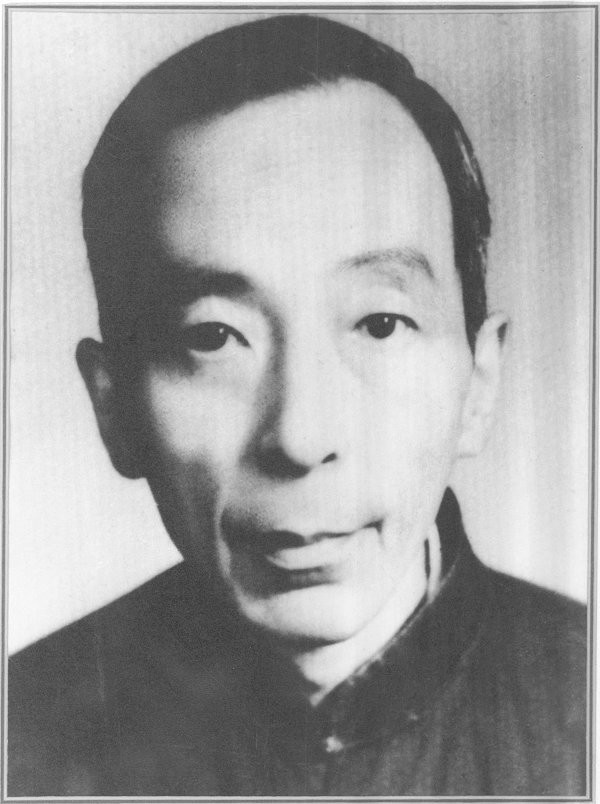
\includegraphics{images/PaoluXu.jpg}
				}
				%\includegraphics[scale=1.0]{figurefile}
				\caption{许宝騄}
				\label{fig:campus}
			\end{figure}
		\end{column}%
		\hfill%
		\begin{column}<0->{.6\textwidth}
			到现在,概率统计课已经进行了一半,我们在这里介绍一下我国非常著名的概率统计学家——许宝騄先生.应当说,他是我们国家概率统计事业的奠基人.
			
			\textbf{A、出身钱塘许氏}
			
			许宝騄(1910—1970年),字闲若,祖籍浙江杭州,1910年9月1日生于北京,因此小名京生。
			
			许宝騄在中国开创了概率论、数理统计的教学与研究工作。在奈曼-皮尔逊理论、参数估计理论、多元分析、极限理论等方面取得卓越成就,是多元统计分析学科的开拓者之一。其研究成果推动了概率论与数理统计的发展。 至今“许方法”(多元分析统计学家谢菲H.Scheffe称之为“数学严密性的范本”)仍被认为是解决检验问题的最实用方法。
		\end{column}%
	\end{columns}
	
\end{frame}

\begin{frame}
	$\quad$许宝騄是20世纪最富创造性的统计学家之一,也正是许宝騄拉开了中国概率论与数理统计学科研究的帷幕,他被公认为在数理统计和概率论方面第一个具有国际声望的中国数学家。《中国大百科全书 数学》称赞说:“许宝騄是中国早期从事数理统计学和概率论研究并达到世界先进水平的一位杰出学者。” 1983年,德国施普林格出版社刊印了《许宝騄全集》(Pao-Lu Hsu Collected Papers)由斯普林格(Springer-Verlag)出版社刊印,全集是由钟开莱主编的,共收集了已发表的、未被发表的论文40篇。书评中有这样一句话:
	
	“许宝騄被公认为在数理统计和概率论方面第一个具有国际声望的中国数学家”。
	
	许宝騄的像片悬挂在斯坦福大学统计系的走廊上,与世界著名的统计学家并列。
	
	$\quad$许宝騄是二十世纪和华罗庚、陈省身齐名的中国数学家,中央研究院第一届当选的5名数学所院士之一(注:另外四位首届数学院士是姜立夫、陈省身、华罗庚、苏步青)。当然由于各种原因的结果,他并不为国人所知。
\end{frame}

\begin{frame}
	$\quad$许先生出身于杭州的名门望族。据许氏家谱记载,杭州许氏本姓沈,始祖是富阳的沈显荣,1536年他在北京经商病故,遗有两子由杭州的表姑夫许魁带回杭州抚养,改姓许,入籍杭州。其中尤以横河桥支系的“积厚轩”堂兴旺。 
	
	$\quad$乾隆三年许家出了第一位举人许钺,之后钱塘许姓一族显宦至多,嘉庆、道光、同治间最盛。许氏十世祖许学范为乾隆三十七年(1772年)进士。许学范生得八个儿子,按照“学乃身之宝、儒以道得民”的行辈排下来,这八个儿子便被时人称人钱塘“八乃”,其中乃济、乃普、乃钊三子为进士,其余四子也皆中举人,皇帝给许家赐匾“七子登科”,意为许家府上出现过七位有才学的人。当时的学者、书法家梁同书曾写对联“世间数百年旧家,无非积德;天下第一件好事,还是读书”赠与许学范。
	
	$\quad$到光绪二十九年,共出了34位贡生、举人,其中9人中进士。许氏共有140多人次出任清代的大小官员,除江西省没有外,分布全国各省,名震朝野。老杭州都知道以前文武官员路过横河桥时,“文官下轿,武官下马”。就是因为许家有许多大官。
\end{frame}

\begin{frame}
	$\quad$许乃济(1777年—1839年),字叔舟,号青士,为嘉庆十四年(1814年)进士。选庶吉士,授编修。嘉庆二十五年(1825年)任山东道监察御史。道光三年(1823年)任兵科给事中。道光五年(1825年)任广东肇罗道,七年(1827年)改广东督粮道,道光九年(1829年)改高廉道。道光十三年(1833年)任光禄寺少卿,官至太常寺少卿。
	
	$\quad$许乃普(1787年—1866年),字贞锡,号滇生嘉庆二十五年(1820年)殿试高居一甲第二名(榜眼),赐进士及第,授翰林院编修。官至吏部尚书。同治五年(1866年)卒,谥文恪。工书,法二王,与祁寯藻、陈孚恩、赵光并称四书家。许乃普子彭寿为道光二十七年(1847年)丁未科会元,殿试位列二甲第一名(传胪)。选翰林院庶吉士。散馆授编修。官至内阁学士。
	
	$\quad$许乃赓为嘉庆二十二年(1817年)丁丑科二甲进士。改庶吉士,散馆授编修。历官右庶子。
\end{frame}

\begin{frame}
	$\quad$许宝騄的曾祖许乃钊(1799年-1878年)行七,字贞恒,号信臣,又号恂普,为道光十五年(1835年)殿试二甲、朝考一等第十名,授编修。之后历任国史馆总纂官,河南、广东学政,内阁学士兼礼部侍郎衔,江南大营帮办。咸丰三年(1853年),出任江苏巡抚,镇压上海小刀会起义,次年因无功被革职。咸丰七年(1857年),以三品顶戴帮办江南军务,咸丰八年(1858年),迁光禄寺卿。咸丰十年(1860年),太平军破江南大营,攻克苏州、常州,再次被革职。不久引疾回乡。光绪四年(1878年)卒。
	
	$\quad$许乃钊的子辈许祐身是许宝騄的祖父,累官至苏州知府。许宝騄父亲许引之从清朝末年至北洋政府时期一直担任中层官员,曾任清朝两浙盐运使。母亲程时嘉,江西新建人。
\end{frame}

\begin{frame}
	$\quad$许家为官当中有两人与慈禧60大寿和死亡有关。
	
	$\quad$许庚身(1825年-1893年),字星叔,号吉珊,崇尚天文、算术、舆地诸学。咸丰二年举人,考取内阁中书。同治元年,以在任官员的身份中进士,任内阁侍读。许庚身在军机处任职近三十年,曾参与策划对太平军和捻军的军事行动。同治十二年,任光禄寺卿。光绪五年,升任礼部侍郎,后分别任户部侍郎和刑部侍郎。中法战争爆发,许以刑部侍郎身份任军机大臣,兼总理各国事务衙门大臣,坚持以“驭夷无上策,可羁縻,不可迁就”的态度对待法国。十四年,升兵部尚书。
	
	$\quad$许庚身曾奉命总办慈禧60大寿,但是在寿前去世,清廷晋赠太子太保,谥恭慎。
	
\end{frame}

\begin{frame}
	$\quad$许宝蘅,光绪二十七年举人。他任军机章京时,记了许多日记,成为研究清末衰亡的重要史料。在光绪、慈禧死亡时,他记载了他忙碌的一天。早上五时,他至西苑门吉祥桥时,知道光绪于昨天酉时死了。进内宫后知道,昨天已颁发遗诏,传位于醇亲王之子,由摄政王监国。等到其他大官到场后,由他拟旨尊慈禧皇太后为太皇太后,皇后为皇太后。然后是拟各种皇太后的谕旨。不料,11点慈禧病危。又拟旨由摄政王面请皇太后掌管大事。下午2点,慈禧换衣,随即死亡。他在日记中说“十一时中两遘大丧,亘古所未有,所谓奇变。”就是说,在11个钟头里,皇室死了两人,真是前所未有的大变故,他说在写各种旨章时,“心震手颤,莫知所主”。可见当时朝廷的慌乱。 
	
	$\quad$根据许宝蘅日记,在选择新皇帝的纪元年号时,最初拟出四个:宪昌、宪治、宣统、圣宪。一般按清惯例,应首选排在前面的“宪昌”,但不知何故,皇太后圈了“宣统”,在临抄写时,重新把“宣统”列在第一位。	
\end{frame}

\begin{frame}
	$\quad$许祐身的孙子一辈也多为知名人士,宝字辈共有兄弟姐妹七人,其中许宝驹、许宝騄、许宝骙被称为“杭州许氏三杰”,许宝驯工于书画、昆曲,是著名学者俞平伯的夫人。一子许宝朴过世较早,但其子许儒鸿却承其世家之风,成就了一代文史兼攻的作家,他便是《慈禧全传》、《胡雪岩》等历史小说的作者、台湾著名作家——高阳。
	
	$\quad$许宝驹(1898-1960),字昂若,北大国文系毕业,曾积极投身五四运动,历任中国国民党一大代表、国民革命军第十八军党代表、浙江省政府秘书长、铸币局局长、国民党中央执委等职。民盟创始人和领导人之一。1949年后,历任民革中央常委、全国人大代表和政协委员。
	
	$\quad$许宝骙,1909年4月1日生于浙江杭州,1932年毕业于燕京大学哲学系,后在广州、北京多所大学任教。抗日战争爆发后,他积极追随中国共产党,投身于抗日救亡运动,是“中国民主革命同盟”的重要发起人之一。
\end{frame}

\begin{frame}
	$\quad$1945年,许宝骙任《正报》主笔,参与“三民主义同志联合会”地下组织,并在争取北平和平解放的过程中开展了积极有效的工作。新中国成立后,许宝骙同志继续在北京任教,同时担任民革中央宣传部副部长、民革北京市委员会代理秘书长。译有穆勒《论自由》、培根《新工具》等。
	
	$\quad$七子登科的同时,还有五凤齐飞入翰林,许佑申的姐姐嫁给了礼部尚书廖寿恒,妹妹嫁给了晚清直隶总督陈夔龙。
	
	$\quad$通过联姻,钱塘许家有许多社会名流姻亲,其中包括俞樾。俞平伯的高祖俞樾(1821-1907)是清朝大学者,浙江德清人,道光进士,官翰林院编修,著有《春在堂全书》二百五十卷。俞樾的二女儿俞绣孙嫁到许家,成了许宝騄的祖母(祖父许佑申),许宝騄的父亲是许引之。许宝騄的一位姑姑是俞樾的孙媳妇,也是俞平伯的母亲。许宝騄的长姊许宝驯工书善画,并善于昆曲,1917年嫁给了著名学者俞平伯。许、俞两家乃故家故亲。许宝騄在家排行第七。许俞两家是亲上加亲,按现代优生学的观点来看,是不符合优生学原理的,值得庆幸的是在两家后代中并没有发生不幸,其后代皆学有所成。
\end{frame}

\begin{frame}
	\textbf{天赋异禀}
	
	$\quad$许宝騄的父亲许引之一生仕宦于晚清、民国,因此幼年的许宝騄随父母出生、成长于宦所。2岁时随家移居天津,八岁时去杭州。1924年,许宝騄十四岁时,父亲病逝于杭州,母亲携全家迁回天津,第二年,移居北京。
	
	$\quad$许宝騄从小体质就比较羼弱,而其慧敏之秉赋已隐然可见。从5岁开始,许引之就请来家庭教师教授许宝騄在家读书,第一位启蒙师为张 树之先生;后改从吴县高德馨(字远香)先生、蕲春陈先生,一直到他十四岁止。期间,许宝騄通读四书五经,涉猎四史及古文辞,大都能琅琅背诵。10岁后许宝騄就学作文言文,因此他的文学修养很深,用语、写作都很精练、准确,塾师评为“简老”。11岁时许宝騄写过以《花生姻缘》和《神花》为题的文言小说。
	
	$\quad$许宝騄学写小楷后,临摹《玉板十三行》,古朴神似。后来为姐夫俞平伯手写的《古槐书屋词》,有刻本行世。又善就古书诗曲小说制作灯谜,颇具巧思。他善于巧妙地利用古文诗词制作灯谜。
\end{frame}

\begin{frame}
	$\quad$十一岁时,许宝騄开始学英文、算术,塾师为杭县邵家驹(字昂士)先生,两年后便能阅读英文的古典文学名著。
	
	$\quad$	许宝騄在幼年之时就已经在数理方面显露出异于常人的天赋。
	
	$\quad$许宝騄在孩提时就能拼摆“益智图”。到北京后,为了能够考取中学,需要从头开始系统补学新式数学知识,为此专门聘请北京大学数学系吴缉熙老师讲授代数及三角,从头起步,仅仅花了连个月的时间就已经成绩斐然,由此也让许宝騄对数学引起极大的兴趣,其数学天才开始崭然显露。
	
	$\quad$1925年暑期后,许宝騄顺利考入北京汇文中学高中一年级。高中学习期间,许宝騄利用暑假时间跟着表姐夫徐传元先生(字孟轮,毕业于美国麻省理工学院)钻研数学,得其指点,进步神速。还坚持学习法文,两年后他的法文达到能会话和作短文的程度。
	
\end{frame}

\begin{frame}
	$\quad$清康熙二十九年,褚稼轩《坚瓠集》中载有“移棋相间法”,最初始于清顺治六七年。清末,经学大师俞樾和夫人在闲暇十之时,也做移棋之试,曾推至二十棋子,并作诗记载此事,诗云:
	
	闲将棋子试推移,黑白分明亦一奇。此后空留遗法在,更谁灯下运灵棋。
	
	(注):褚稼轩《坚瓠集》有移棋相间法,以黑白三子,三移而黑白相间,自三子至十子皆然内人复推广之,自十一子至二十子,今存其法于《春在堂随笔》。
	
	$\quad$许宝騄在中学读书的时候和俞樾的曾孙俞平伯根据《春在堂随笔》记载,又设法查找《坚瓠集》,知道了最初之法,他们就研究推增至五十子。以后并非不能再推加,因过于繁琐而止。一年后,许宝騄以研究所得移棋相间“合四为一”的新律相告,俞平伯先生有一段文字记此事,文曰:
	
	$\quad$已已新正二日之夜,忽以电话觅谈,适余外出,越曰访之,乃以合四为一之新律相告,其法简而整,其言明且清,虽其根柢不出四律,而去其繁冗,正其谬误,使人一览豁然贯通,于应用上方便至多,……依新律,则口耳授受一分钟可毕,真庶乎儿童不乱矣。
	
\end{frame}

\begin{frame}
	$\quad$清初以来的“移棋相间法”,本是一种有数学性质的游戏,许宝騄与俞平伯先是推至五十棋子,以后又总结出四条规律,本来还想成一公式,后来许宝騄因为赴英国留学,科学研究任务繁重,对少年时代的游戏也就无暇再问了。
	
	$\quad$1928年,汇文中学毕业后的许宝騄考入燕京大学理学院学习化学。当时考大学是各校单独命题考试招生,许宝騄当时报考的是燕京大学和清华大学。按许宝騄当时的水平和成绩考入清华大学是没有问题的。不过因为许宝騄文笔快捷,思想敏锐,当时,有不少认识他的人问他题目怎样做,他帮助别人做题而耽误了自己,因而清华大学没有录取,而被燕京大学录取了。
	
	$\quad$许宝騄在中学期间因为受表姐夫徐传元的影响,对数学颇有兴趣,入大学后了解到清华大学数学系最好,决心转学念数学。由于出众的才能,1929年就转入清华大学数学系继续深造,仍从一年级读起,一起学习的有华罗庚、柯召等人。
	
\end{frame}

\begin{frame}
	$\quad$著名数学家、国际数学界最高荣誉“菲尔兹奖”获得者丘成桐坦言,从1927年到1949年清华数学系是全国最好的数学系。当时清华可算中国数学的一个学术中心,学校当时请了两个著名的外国教授,其中之一便是维纳,清华面向全国办数学培训班,培养了一批教员。

	$\quad$当时清华的教授有杨武之、熊庆来等。杨武之就是杨振宁的父亲,他是一位家教很严的父亲,有时甚至杖责儿子,听说一度因此而使父子关系紧张。
	
	$\quad$杨武之教授自认学术声望不算高,当时,杨武之公开承认自己的数学成就、解题能力不及他的学生,但他认为解不出难题的教授也可以培养出杰出的学生,因为老师知道哪些题难,哪些题重要,可以布置给学生去想。许宝騄等数学家也许正得益于在清华的这些训练,据华罗庚后来回忆,当时他们一个班有约40人,这门课老师出了几道难题,他(华罗庚)就上图书馆查题鉴、查参考书,向助教请教,每天晚上开夜车,匆匆忙忙完成才发现当天就要交作业了,每次都以为只有他一人按期交作业并得全分,但发下来的,才发现每次都是四个人,另外三人就是陈省身、许宝騄、柯召。
	
\end{frame}

\begin{frame}
	$\quad$许宝騄在清华读书,成绩十分优秀,熊庆来,杨武之等对于他的才华十分看重,杨武之曾作诗书赠先生,首句即为:“许公宝騄,颇有天才”。

	$\quad$许宝騄除了数学特别出色之外,兴趣爱好十分广泛。许宝騄受家庭熏陶,爱好昆曲,工昆旦兼习小生,会拉二胡,精善音律。每听一曲,不出几遍就能写出谱子,表现出良好的艺术才能。30年代,许宝騄与姐夫俞平伯共组清华谷音社。解放后,在教学科研之余,经常参加老君堂俞宅昆曲清唱和北京昆曲研习社活动。
	
	$\quad$许宝騄还是桥牌高手,当时西方的桥牌刚刚传入清华,所以很多人对打桥牌这种娱乐形式很感兴趣。许宝騄更是利用业余时间钻研桥牌方面的书籍,以至于精通桥牌,牌艺出众,在西南联大任教时曾参加清华的校队,经常参加比赛,还常和朱自清、浦江清、俞平伯在俞家打桥牌。
\end{frame}

\begin{frame}
	\textbf{双博士}
	
	$\quad$许宝騄幼年体质就非常虚弱,以至于对他后来的工作生活造成了很大的影响。在清华读书时时,体重还不到40公斤,并且患旅游肺病和胃病,肺病需要加强营养,但因为同时有胃病,营养得不到吸收。许先生体育成绩大概不及格。当时可用庚子赔款去英国留学,许宝騄所在的清华大学每年有一名额,这当然是非许宝騄、华罗庚莫属。
	
	$\quad$1933年,许宝騄于清华大学毕业获理学士学位,经考试录取赴英留学,体检时发现体重太轻不合格,未能成行。
	在这种情况下,许宝騄到香山疗养过一段时间,当时住在香山脚下的一所房子里,期间注意营养,加强锻练,使身体状况大为好转。
	
	$\quad$1934年许宝騄进入北京大学数学系担任正在访问北京大学的美国哈佛大学教授奥斯古德的助教,前后共两年。奥斯古德是分析方面的专家,在他后来出版的书中,提到了许宝騄的帮助。在这两年内许宝騄做了大量的分析方面的习题,并进行了一些研究,于1935年发表了两篇分析方面的论文,其中一篇是与江泽涵合作的。那时芬布尔和阿蒂肯合写的《标准矩阵论》已出版,许宝騄熟练地掌握了矩阵的工具,尤其精通分块演算的技巧。所以这两年内他在分析和代数两方面都打下了扎实的基础。
\end{frame}

\begin{frame}
	$\quad$1936年许宝騄再次考取了赴英留学,派往伦敦大学学院,在统计系学习数理统计,攻读博士学位。
	
	$\quad$上世纪三十年代,统计学,特别是各种专业统计,例如生物统计、医药统计、农业统计、工业统计首先在英国迅速发展,得到广泛的应用。许宝騄在英国伦敦大学学院攻读博士学位期间,师从著名统计学家Neyman。此后的几年间,他在统计推断和多元分析等方面做了一系列理论性开创性工作,把许多数学中的分支,如矩阵论、函数论、测度论等引进统计学,使统计学中的许多问题的理论基础更加深厚,逐渐形成了统计学中的一个主流方面——数理统计。在新中国成立后的相当长的一段时间里,在研究机构和一些大学里,统计学往往被称之为数理统计。其实把数理统计视为统计学的一个主要分支似乎更妥当些,可以说,许先生是数理统计这一方向的奠基人之一。
\end{frame}

\begin{frame}
	$\quad$1936年到1940年,伦敦大学学院统计系正处于鼎盛时期,是公认的数理统计研究中心。该系名家汇聚,皮尔逊退休后,由费歇任高尔顿实验室主任,皮尔逊当系主任。一些学者陆续前来访问,包括美国的多元分析专家霍太林,威尔克斯,频率曲线专家克莱格,概率专家费勒。教师中有内曼这样的教授,所以许宝騄很快就接触到数理统计方面科学前沿的情况。自30年代到40年代,正是N.P.理论(内曼-皮尔逊理论)的形成时期。对于点估计和假设检验,首次提出优良性的概念,明确地提出了应该寻求优良的方法,而优良性有客观的标准。

	$\quad$1938年许宝騄导出了霍太林提出的T2检验在一定意义下是局部最优的,主要的困难是在零假设不成立时,如何导出T2的分布,通常称为非零分布,有了非零分布才能讨论功效函数的大小。他的这一工作在N.P.理论和多元统计分析中都是占有重要地位的先驱性工作。
	
	$\quad$内曼(Neyman)是著名统计学大师,在其一生中,与许宝騄相遇两次。1936-1938年,在英国大学学院时,内曼是许的老师。他后来称许是他最好的学生。1945-1947年,许先生去美国时,他们又相遇了。
\end{frame}

\begin{frame}
	$\quad$内曼在纪念许宝騄的文章中写了如下的这一段话来论述这篇论文的意义: 
	
	$\quad$“这篇文章开创了两个发展方向。一方面,他的学生席玛卡将许的方法用于多元问题(霍太林的T2及多元相关系数)……。另一方面,在这篇文章中,许提供了获得全部相似检验的新方法。在许的建议下,席玛卡和莱曼将这个方法用于其他问题,后来莱曼和谢飞形成了完备性的概念。” 
	
	$\quad$这足以说明许宝騄在这一方面的工作对后来的研究有多大的影响。
	
	$\quad$1938年许宝騄共发表了3篇论文。当时伦敦大学规定数理统计方向要取得哲学博士的学位,必需寻找一个新的统计量,编制一张统计量的临界值表,而许宝騄因成绩优异,研究工作突出,第一个被破格用统计实习的口试来代替。1938年他获得了哲学博士学位。
	
\end{frame}

\begin{frame}
	$\quad$同年,系主任内曼受聘去美国加州大学伯克利分校,他推荐将许宝騄提升为讲师,接替他在伦敦大学讲课。1939年,许宝騄又发表了两篇论文,1940年又发表了3篇。其中两篇文章是数理统计学科的重要文献,在多元统计分析和内曼-皮尔逊理论中是奠基性的工作,因此他获得了科学博士的学位。
	
	$\quad$许宝騄在30年代做的论文,被一些人士认为他可能是继费歇(Fisher)之后执掌统计大旗的人,但是以为身体很差的缘故,学术工作不能不受到一些影响。所以,后来成就就稍逊于皮尔逊(Pearson)和内曼(Neyman),但不可否认许宝騄是世界第一流的统计学家。
\end{frame}	

\begin{frame}
	\textbf{执教西南联合大学}
	
	$\quad$1940年,抗日战争处于最艰难的时候,在英国伦敦大学学院获得双博士学位后的许宝騄,放弃优越的学术环境和生活条件,毅然回国效劳,受聘为北京大学教授,于1940年到昆明,在西南联合大学任教。
	
	$\quad$当时昆明的工作条件和生活待遇极端艰苦,单身耽在昆明的许宝騄在那段时期的生活是十分艰苦俭朴的。他住一间宿舍,既是卧室又是书房,除了书桌、床铺和一块大黑板外,别无其它大型家具。在这种艰难的环境下,许宝騄喜欢穿一件风雨衣出外散步,在校园附近漫步时学生们常能看到他的儒雅风度。
	
	$\quad$战争年代生活是十分困难的,1943年-1944年许宝騄给Neymann的信中曾提到过挨饿之事,但他仍然坚持研究。
	
\end{frame}

\begin{frame}
	$\quad$当时的西南联大图书资讯极端贫乏,连教材都少有,学生听课主要靠 记笔记。许宝騄学习非常勤奋、刻苦,因为资料贫乏,以至于想找一本书都困难,他曾手抄过梯其马舍的整本《函数论》,他念过的书, 往往都写了不少批注,有的书都被他翻得成零页了。
	
	$\quad$在1941年到1945年抗日战争胜利,许宝騄在“Biometrika”、“J. London Math. ”、“Ann. Math. Statist。”……等许多国际权威性刊物上发表了十多篇有关数理统计等方面的开创性文章,成为国际上数理统计这一方向的奠基人之一。他曾经说过,我们在某杂志上发文章,不是借该杂志来标榜我们的学术水平,应该让我们在该杂志发表了文章来抬升此杂志的地位。先生这样说了,也确实这样做了。
	
	$\quad$在西南联大期间,许宝騄对Neyman-Pearson理论作出了重要的贡献,他得到了一些重要的非中心分布,论证了F检验在上述理论中的优良性,这些都是奠基性的工作;同时他对多元统计分析中的精确分布和极限分布得到了重要的结果,导出正态分布样本协方差矩阵特征根的联合分布和极限分布,这些结果是多元分析中的基石。以上这两方面的工作确立了他在数理统计中的国际上的地位。 
\end{frame}

\begin{frame}
	$\quad$此外许宝騄在寻求统计量的极限分布,在次序统计量的极限律型方面,都有重要的贡献。
	西南联大时代,许宝騄开设微分几何课程。
	
	$\quad$当年在西南联大简陋的教室讲课,往往无法听到上下课的摇铃声,而他又没有手表,于是每次上课时他就将装有一只闹钟的布袋放在讲台上。当上课的学生们第一次忽然听到讲台上布袋里铃声大作,而许先生又笑着说了一声“下课了”时,大家真是惊喜交加。
	
	$\quad$许宝騄备课极为认真,讲授条理清晰,擅长于在课堂上强调一些细微之处。更因其出生于书香门第,自幼受过很好的文学熏陶,所以他善于运用形象思维的语言来解释现代数学基本概念产生的必然性。 
	
	$\quad$他对学生说微分几何不过是微积分的一种应用而已,而主要工具是泰勒级数展开,再用一点儿初级代数计算。这些话对学生产生了很大影响。许宝騄在教学中特别强调“直观地理解数学”的重要性,他主张要把数学定理及其证明的“原始思想”告知学生,总是殷切地期望学生能直观地领悟数学命题的来龙去脉。在分析问题时,他强调要有一种“内视”能力,认为“数学中的抽象能力很重要,一些问题经过抽象后,不仅简明而且其实质也清楚了”。
\end{frame}

\begin{frame}
	$\quad$他循循善诱,对学生的指导具体而细致,对学生的读书笔记逐字逐句地修改,甚至错别字和标点也要改正。他批改作业,不但指出正误,而且给出更好的解法。
	
	$\quad$宝騄对做一名好教师有独到见解:“要做一个好老师,必须自己有相当的功底,才能讲好。应该做到以十当一,自己会十,但讲出来的是一。”他说道:“教师在台上讲课,就像举重运动员,应该举重若轻,很重的东西,一下就举起来了,让人看了感到舒服;而不应该是举轻若重,一份很轻的分量,举也举不起,两腿发抖,让人感到难受。”
	
	$\quad$正是许宝騄这种精辟的教学思想,深深地影响了学生。他们中一些人已经成为今日的数学栋梁,如钟开莱、冷生明、王寿仁、徐利治和张尧庭等,以及美国的比乌曼(I.Biumen)、布拉迪(R.Bradiey)、罗宾斯(H.Robbins)、鲍克(A.Bowker)、莱曼(E.Lehmann)和奥利金(I.Olikin)等。
\end{frame}

\begin{frame}
	$\quad$徐利治曾说,他从许宝騄身上学到了“不怕计算”和“乐于计算”的习惯,十分乐于从计算中发现规律和提炼一般性公式。许宝騄的教学风格也给教堂山的美国学生留下了深刻印象。比乌曼写道:“许坚持深入浅出,毫不回避困难,特别是深沉、明确而默默地投身于学术的最高目标和水准,这些精神吸引了我们。”布拉迪说:“许堪称后辈的典范。”罗宾斯回忆道:“许是令人难忘的,无以伦比的。” 
	
	$\quad$在这一时期,许宝騄受群众的影响,加入了一个政治团体——中国民主革命同盟,它是受中国共产党影响的。
	
\end{frame}

\begin{frame}
	\textbf{赴美讲学}
	
	$\quad$许宝騄的老师内曼和小皮尔逊在1933年发表了关于假设检验的论文,把检验问题作为一个数学最优化问题来处理,发展了费希尔的研究工作。由于费希尔对皮尔逊有成见,因而对内曼和小皮尔逊的研究也不以为然,甚至称其编辑的《统计学研究通报》是“一堆破烂货”。这也使得内曼感到在英国难以发展,于1938年4月应聘为美国加州伯克利大学数学系教授,并筹建了统计实验室。
	
	$\quad$1944年的英国正在遭受着德国的轰炸。希特勒亮出了讹诈已久的“秘密武器”——无人火箭。正是在这种情况下,内曼决定回到英国为国效力。但在离开伯克利大学数学系之前找一个适当的接班人是内曼所面临的问题。耐曼始终认为,在战争时期坚持教育质量是非常重要的,美国显然已没有多余的老资格统计学家。二战时期,美国人才紧缺,内曼培养的学生,一个个地被军方调走。在考虑接班人时,想到了他的学生许宝騄。内曼非常器重许宝騄,认为许宝騄是新一代数理统计学家中的佼佼者,一度选定其为接班人。
	
\end{frame}

\begin{frame}
	$\quad$1943年,内曼收到过许宝騄一篇论文的抽印本。中国的形势一片混乱,天下三分,其一在日本人的统治下,其二由共产主义者领导,第三部分属于民族主义者。许宝騄在某处一个地窖里从事科学研究。他的工作居然能够印出来,简直是个奇迹。他渴望到美国来。
	
	$\quad$内曼第一脚踏上赴英的旅程,就给许宝騄发了一份电报,邀请他到伯克利来讲六个月课,并在来年担任一个收入有保证的职务。
	
	$\quad$由于内曼的邀请,许宝騄于1945年八月在北京大学留职停薪,在当年欧战结束之后,赴美参加了伯克利(Berkeley)第一届概率统计的学术交流会。当时,赴美路费是内曼从44年开始设法筹措的。
	
	$\quad$会后,许宝騄在加州大学伯克利分校教了一个学期。在伯克利任教期间,加州大学主要教员有两位,一位是内曼,另一位就是许宝騄。
	
\end{frame}

\begin{frame}
	$\quad$内曼因有许宝騄这样才华出众的数理统计学家在伯克利而感到高兴。因此,当他看到许宝騄在一张表中仅仅被称为统计学讲师后,便对这个“令人不快的错误”向校方提出了抗议。
	
	$\quad$他说:“有人也许会说在一张表格中怎麽称呼关系不大,但是既然写上了头衔就有其目的,否则写它做什麽。对许宝騄来说,在这样的失误中所受到的损害比美国人更多。作为一个中国学者,两所美国的重要大学邀请他来当访问教授,这是一种很高的荣誉。事实上,要是那张表能真实的反映他的工作,那就好了,那样一份东西留在他家中,子孙后代看了也会感到自豪的。”
	
	$\quad$一学期之后,许宝騄又到哥伦比亚大学教了一个学期。当时美国名大学争相邀请许先生去任教,内曼希望许宝騄继续回到伯克利。但最后,许许宝騄决定在哥伦比亚大学的教学工作结束后跟着郝泰林(Hotelling)到北卡罗来纳大学去筹建统计系。
	
\end{frame}

\begin{frame}
	$\quad$许宝騄在郝泰林创办的北卡罗来纳大学的新统计系教了一年。因为统计这个领域正在发展,很缺乏像许这样有成就的学者,他在这三个学校都很有建树。他被选为IMS (Institute of Mathematical Statistics)的委员,这是1946年的事。
	
	$\quad$许宝騄在伦敦大学学院攻读学位时,熟读了克拉美的《随机变量与概率分布》(1937年出版)掌握了特征函数的工具,所以他对极限理论很有兴趣。1947年他与H.罗宾斯合写的论文《全收敛和大数定律》,第一次引入全收敛的概念。当时国际上在概率方面主要的兴趣是独立随机变量之和的极限分布,正在从古典的向近代结果转化。一些著名的概率论专家如科尔莫哥罗夫,辛钦,格涅坚科,莱维和费勒等人都在攻这难题。1947年,许宝騄已获得了主要的结果:每行独立的无限小随机变量三角阵列的行和,依分布收敛到一给定的无穷可分律的充分必要条件。由于当时信息不通,他不知道别人的工作情况,当时他写信给钟开莱时说:“……我担心正在进行的工作会和别人相重……”
\end{frame}

\begin{frame}
	$\quad$后来,他知道了格涅坚科和科尔莫哥罗夫的工作,就没有再发表自己的研究。实际上许的方法和俄国人还是不同的,许的方法更为直接。1968年,当格涅坚科和科尔莫哥罗夫合写的《独立随机变量之和的极限分布》英译本再版时,钟开莱用附录的方式第一次刊印了许宝騄的工作。然而许在生前并未看到这本书,他始终没有看到自己的这一部分工作的公开发表。
	
	$\quad$1947年,许宝騄谢绝了一些大学的聘任,回到北京大学任教授。当许宝騄回国时,内曼一再挽留,想把他争回自己的麾下。回国后,许宝騄也与奈曼保持了多年的联系。许宝騄对科学所做的贡献以及孜孜以求的好学精神,是与内曼的教诲和影响分不开的。
	
	$\quad$1948年,许宝騄当选为中央研究院院士。回国后不久,许宝騄就发现已患肺结核。此后他长期带病工作,教学科研一直未断,在矩阵论,概率论和数理统计方面颇有建树。
	
\end{frame}

\begin{frame}
	\textbf{执教北京大学数学系}
	
	$\quad$许宝騄在北卡罗莱纳大学开创了统计系之后,于47年底回北大数学系任教。
	
	$\quad$许宝騄回国可能也为了结婚,但由于种种原因,他终身未婚。关于他的个人婚姻事宜,有各种说法,俞平伯的儿子俞润民的说法可以认为是可靠的。俞润民先生有一姑父郭则澐,是清朝翰林,曾在北洋政府徐世昌处任秘书长。郭有一女儿,与许先生年龄相仿。按中国旧的传统来说,许郭辈份不合,许宝騄比这位郭女士长一辈。郭则澐认为虽然辈份不合,但郭先生与许宝騄先生的父亲在北洋政府时期是同事,作为儿女之事也是合适的。所以郭先生还是赞同这桩婚事。据推算,1936年许宝騄留英以前,两人已有恋爱关系而往来,后来之所以没有成,是郭先生的儿子(郭女士的弟弟)反对这桩婚姻,欲将他的姐姐嫁给国民党的一个官吏。后来,郭女士嫁给了一个铁路局长。这样,许先生的婚事就告吹了。这件事情发生在抗战时期(40-45),许郭之间相处的时间不长。
	
\end{frame}

\begin{frame}
	$\quad$外面传说,许先生因肺结核未能成婚,这不符合事实,只是对外的一种托辞。另据俞润民回忆,许宝騄在美国时,曾有一女士有意于他,这一次是自由恋爱。据润民回忆,许宝騄给俞平伯先生的信中提到他采取的策略是“以退为进”,现在已搞不清楚以退为进的具体含义。从现在恋爱方式来看,应是双方主动。不久发现身染肺疾,乃复废约。此后终身未娶。
	
	$\quad$许宝騄因为学与统计学的诸多领域成果丰硕,造诣精深。1948年,当我国中央研究院首批评选院士时,三十八岁的许宝騄就高票当选。
	
	$\quad$在1948年辽沈战役后,许宝騄已确信“国民党败局已定”,他很欢欣1949年我国的解放,还拍电报给美国的同事表达他对中国新生的喜悦之情。
	
	$\quad$从1947年至1956年,许宝騄一直在北京大学数学系执教。开设一些国内一般大学不开的课程,像“实变函数论”等,并积极开展多元统计和矩阵论方面的研究,特别是关于矩阵方面所获得的结果,就是基础数学家,也为之赞叹,此乃上上之作。
\end{frame}

\begin{frame}
	$\quad$中共建政初期,不认为概率统计是重要的,他在矩阵论方面的工作,刊登了几篇论文在中国的数学杂志上,发表的论文还有与特征函数有关的内容。1954年,中国科学家代表团访问苏联,柯尔莫果洛夫(Kolmogorov)教授问到了许。人们开始认识到许的国际地位。1955年,他成为中国政治协商会的一名委员。同年他与其他著名的数学家,如华罗庚、苏步青等一起被选为中国科学院学部委员。
	
	$\quad$1956年,周恩来总理主持制定了“全国科学发展12年远景规划”。规划中把概率论与数理统计作为数学的三大重点发展方向之一。为了落实这一规划,大力发展我国概率论与数理统计,许宝騄殚思极虑,费尽心力,采取了当时条件所能做到的一切措施。
	
\end{frame}

\begin{frame}
	$\quad$1956年秋,中科院数学研究所的王寿仁先生,张里千先生,中山大学的郑曾国先生、梁之舜先生被借调到北京大学任教。与此同时,从北京大学数学力学系抽出34名四年级学生,从中山大学和南开大学各抽调10名四年级学生来北京大学培养,此外北京大学还接收全国各主要综合大学的概率统计方面的教师来进修。许宝騄亲自主持“独立随机变量族的极限理论”的讨论班,系统地学习了“测度论”、“概率极限理论”、“马尔可夫链”、“数理统计”等课程。这是我国第一批培养的数量可观的概率论与数理统计人才。自此以后,全国各综合性大学绝大多数都设有概率论与数理统计教研室。
	
	$\quad$1958年以后,先生主持着三个讨论班:数理统计、马尔可夫过程、平稳过程。参加讨论班的人员,不仅有北京大学概率论与数理统计教研室的师生,还有校外的一些人士。
	
\end{frame}

\begin{frame}
	$\quad$在1956年第一批大规模培养概率论与数理统计人才的实践基础上,许宝騄逐步确定了本专业的必学的基本课程:测度论;概率极限理论(后改称分析概率论);随机过程论;数理统计。根据本专业的不同研究方面,可在下列诸课程中选择一两门:马尔可夫过程,平稳过程,博奕论,排队论,统计试验设计,抽样论……等等。
	
	$\quad$1956年以前,北京大学数学力学系仅开设一门概率论课程,教材是苏联Gnedenko所著“概率论教程”(丁寿田译)。此书作教学参考书可以,完全作教材并不太合适。许先生建议搞教材建设,一是引进,翻译国外一批优秀著作当教学参考书,二是组织力量自己写书。
	
	$\quad$遗憾的是,由于“文革”前以阶级斗争为纲,这些著译计划,在许宝騄有生之年以前,绝大部分没有完成,有的仅出了一半就夭折了,有的还在酝酿中,等到“文革”后,才出版了一部分。
	
\end{frame}

\begin{frame}
	$\quad$“文革”前,我国与西方并无学术交流,许宝騄计划在1957和1958两年聘请苏联和东欧的一些著名学者来华讲学。计有:苏联的Denkin教授,Prokhorov教授,波兰的Fisz教授和Urbanik教授。结果,1957年Fisz来北京大学讲了多元分析和抽样论等专题;Urbanik来北京大学讲了广义随机过程;Denkin于1958年来北京大学讲了马尔可夫过程的几个前沿课题。由于当时反右和大跃进运动,基本上没有取得什么效果。
		
	$\quad$49年以后,国内教学方面的杂志,除了少数几所大学的学报以外,就只有“中国科学”、“科学纪录”、“数学学报”和“数学进展”这几种主要杂志。年青人的文章很难有发表的机会。有鉴于此,许宝騄极力主张创办概率统计杂志。还说,如经费不够,可从我的积蓄中资助。无奈那时对出版物的控制很严,就连与政治相隔甚远的杂志也不易获得创刊。
\end{frame}

\begin{frame}
	\textbf{无言的结局}
	
	$\quad$从1956到1959年,在许宝騄的领导下,不变原理 (Prokholov,Donsker的论文)、多元分析(Anderson的书)和随机过程(Doob的书)是他所主持的讨论班讨论的主题。他要求他的学生在讨论班上主讲,在他们讲完后,他再用他特有的简洁的方法给以总结。从1959到1962年,试验设计、抽样调查(cochran书)都是研究的主题。在他领导下,这一阶段做过林业的调查。从1963到1966年,主题是次序统计量、平稳时间序列(Grenander和Rosenblatt的书),马尔可夫过程以及组合数学。
	
	$\quad$从 1955年起,许宝騄身体非常虚弱。他于1933年开始患肺结核,后来终身未娶,过单身生活。他约有174公分身高,但体重只有43.2公斤。到了六十年代,那时他已因身体条件不能在课堂上讲授概率论。而后的岁月,他只能在家中坐在沙发上对讨论班的研究集体讲课。
\end{frame}

\begin{frame}
	$\quad$当1966年5月文化大革命冲击来临后,所有的教学活动都停止了,他和学校中其他的同事都遭受到折磨。
	
	$\quad$从北京大学办公楼往东南行约五六百米,柳林深处坐落着几栋小平房,有的形似老北京的四合院,有的由门字形的三排平房组成,这就是鲜为人知的佟府。
	
	$\quad$许宝騄从上世纪五十年代初到1970年他去世,就一直住在佟府丙八号。这是一所两廊四间的小平房。一进门是一个临时封闭起来的托檐,不到四平方米,用作厨房。由此前进,是一条由北向南的走廊,尽头是一间贮藏室,东西两侧各有两居室。西侧较大,住着张景昭老师一家,东侧两间较小,进门一间大的,也只有十三四平方米,算作是许宝騄的客厅,里面的套间就是卧室和卫生间了。客厅其实是一个多功能厅。厅内东面墙上,挂着一块黑板,北面放着两个齐屋顶高的书架和一把双人沙发,西南各放置一把单人沙发,中间是一张一米见方的矮桌,厅内还放着几张小凳和几个竹壳热水瓶。许宝騄主持教研室的讨论班时,这个客厅就是教室;教研室要政治学习或讨论问题时,它变成了小会议室;查阅资料时,它变成了图书馆;用餐时,它又变成了餐厅;只有外客来访或学生向先生问问题,这间小屋才恢复原来的角色——客厅。
	
\end{frame}

\begin{frame}
	$\quad$许宝騄饮食非常简单,一天三小瓶牛奶,早中晚各一瓶,中餐和晚餐也只有两三碟小菜,由于先生不仅患过肺病,还有胃病,食量很小。张景昭老师曾在西南联大数学系就读,许先生当时是西南联大教授,所以张也可算许先生的学生,为了照顾许先生,她与许宝騄合请一个保姆料理家务,并经常陪先生一起进餐。由于房子小,保姆只能早来晚归。

	$\quad$许宝騄绝大部分时间在卧室工作。靠坐在床上,在一块一尺见方的薄板上把稿纸展开,撰写论文和讲稿。由于睡眠情况不好,黎明前就开始工作,晚上无人照顾,饿了就用一块巧克力和一杯热开水充饥,“三年困难期间”,巧克力也随之困难掉了。累了就听听收音机,然后再睡一会。卧室中总是放着一台“熊猫牌”收音机,这是了解时事和休闲的主要工具。
	
\end{frame}

\begin{frame}
	$\quad$上世纪五十年代,许宝騄寒暑假还到北京城内的宾馆疗养一两个星期,六十年代以后,几乎是足不出户。自患肺病后,身体一直瘦弱,无论春、秋、冬,在室内总是穿着长衫和毛裤,只有外客来访,才着正装。
	
	$\quad$没有多少人知道,住在这样简朴的居室,过着如此清贫的生活,忍着如此的孤寂,竟然是为我国科学事业辛勤耕耘一生的一代学术宗师许宝騄先生。
	
	$\quad$文化大革命中许宝騄并未中断研究,当时看不到任何杂志,直到1970年,才允许他看杂志,那时他已瘫痪。在两个月内,他翻阅了1966年“文化大革命”以后的全部《数理统计纪事》,了解国际上的学术动态,写下了最后一篇关于BIB与编码的论文,并将这篇文章的手稿托付给段学复教授。
	
\end{frame}

\begin{frame}
	$\quad$1970年12月18日许宝騄去世。临终时,在他枕边搁着一枝他用了数十年的派克笔,从床头到地板散落着一大堆演算的草稿。这些遗物,见证了先生临终前一刻还在继续着他终生的事业,还在思考和探索广阔无垠的科学世界。
	
	$\quad$去世时,身边无一亲朋好友。一代宗师,竟这样走完他的人生之旅。虽然他患过肺结核和胃病,但这些均非不治之症,更何况50年代末已治癒。若不是那场“史无前例”的运动,先生何至英年早逝,六十而亡。一位终身独居,为国家的科教事业而呕心沥血的爱国者,一位享誉国内外的学术泰斗,仍难逃此劫难,实为我们国家的不幸,民族的不幸。
	
	$\quad$如今的佟府丙八号,早已是人去房毁,若仅是人去房空,还可以去那里凭吊先生,现在,只能把崇敬和谢恩之情永铭心间。
\end{frame}

\begin{frame}
	$\quad$许的确是中国统计学家的先驱,他开创了这条道路。他被公认为在概率统计领域具有国际地位的首位数学家(见Springer-Verlag出版社1983年刊印的许宝騄全集)。许宝騄的像片悬挂在斯坦福大学统计系的走廊上,与世界著名的统计学家并列。
	
	$\quad$奈曼认为,许绝对地是与阿伯拉罕、瓦尔特 (AbrahamWald)具有同一水平的人,他们是他下一代中两个杰出的数理统计学家(见Reid书奈曼传)。瓦尔特是在1950年到印度旅游演讲后死于飞机失事,才48岁。许死时60岁。不幸的是许在1950年后未能发表更多的卓越的论文,但他确实给中国统计的发展打下了坚实的基础。
	
	$\quad$80年代中期,在旅美华裔统计学家郑清水的协助下,曾由德国Springer出版社委托钟主编出版了英文版的《许宝騄选集》。无疑,这是对世界统计数学文库的重要贡献。后来又在钟开莱、郑清水、徐利治联名倡议下,创立了“许宝騄概率统计数学奖”,并且发布了一次奖。但终于由于基金匮乏和人力不济等原因,未能使这项具有深远意义的数学奖顺利地继续运作下去。 
	
\end{frame}

\begin{frame}
	$\quad$他不仅自己在多元分析方面有很多开创性的工作,他还培养了像安德森、奥肯等国际上多元分析学术带头人。
	许宝騄先生把数学家分成三流,他说:
	
	$\quad$“第一流的数学家,是有天才的,他们能开闯新的领域,如柯尔莫哥洛夫,冯.诺依曼,维纳这一类人,这些人是可望而不可及的。
	
	$\quad$第二流数学家是靠刻苦学习而成的,认真消化整理前人的东西,在这个基础上有所创造发现,象欣钦这样的数学家就是这一类的,他写的《公用事业理论的数学方法》、《信息论基础》等就是消化整理的结果。这种工作对后人影响较大,年青人可以在这个基础上较快地进入科学的前沿,中国缺少一批做这一类工作的人。
	
	$\quad$第三流的数学家只在某一、二个问题上有一点贡献,不能象第二流的那样有系统的工作。剩下的就是不入流的数学家了。”
	
\end{frame}

\begin{frame}
	$\quad$他认为自己没有才能,是刻苦学习得到的,他也没有经验去培养有天才的人,他只能传授如何认真学习,努力钻研,埋头苦干的经验。他衷心希望他的学生超过他,一次他在讨论班上说:“自古以来,只有能教出状元来的老师是光荣的,至于做状元的学生那就没有什么了。”
	
	$\quad$许宝騄的大弟子钟开莱和许一样也是一位才智出众的人物。他俩出生于历史名城杭州市,都对中国古典文学有深深的爱好和素养,他俩都能写出典雅的中文文章和英文文章。可以这么说,是许宝騄造就了钟开莱,若没有许宝騄的提拔,钟开莱恐怕就难以成名。钟开莱在中学时成绩很好,以双百、第一的成绩考进了西南联大,在大学期间成绩也很好,师从华罗庚研究数论。但钟与华都较自负,两人关系不很融洽,华罗庚出的论文题钟觉得不满意,钟就自己找题做。据说他们在讨论数学问题时,都曾拍案而起,互相反问“你有什么了不起?”学位答辩时,结果是全票通过。之后,询问导师的意见,决定他是否留校,华罗庚立即回答“不留”,但许宝騄马上说:“你不留我留”。一般来说,如果一个教授决定不留某一学生,别的教授不便再留,但许先生实在爱惜钟的才华,又知华、钟二人关系不好,结果钟开莱改从许先生。
	
\end{frame}

\begin{frame}{Research}
	$\quad$\begin{tabular}{|l|l|l|}
		\hline Years & where & Topics  \\
		\hline 1935 & Beijing & topology \\
		\hline 1938-1940 & London & statistics\\
		\hline 1941-1945 & Kunming & Random matrices \& Limiting distr.\\
		\hline 1946-1947 & USA & Matrices \& complete convergence \\
		\hline 1949-1964 & Beijing & Ch.f., Matrices trasf.,Markov processes, \\
		\hline & &  Experimental design \& Limiting distr. \\
		\hline 1968- & - & Markov chain,Random Mat.,\\
		\hline & & Limiting distr., Coding. \\
		\hline
	\end{tabular}
\end{frame}

\section*{常见分布总结}

\begin{frame}{离散均匀分布$\quad$Discrete uniform distribution}
	集合$\{a_1,\cdots,a_m\}$上的离散均匀分布,其中$m\in\mathbb{N}_+,a_j\in\mathbb{R},j=1,\cdots,m$
	
	\begin{itemize}
		\item 分布律$P(X=x) = m^{-1},x = a_j,j=1,\cdots,m.$
		\item 数学期望$\mathrm{E}X = \overline{a} = \sum_{j=1}^m a_j/m.$
		\item 方差$\mathrm{var}X = \sum_{j=1}^m (a_j-\overline{a})^2/m.$
		\item 概率母函数$g(s) = \sum_{j=1}^m s^{a_j}/m.$
		\item 特征函数$\phi(t) = \sum_{j=1}^m e^{ia_jt}/m.$
	\end{itemize}
\end{frame}

\begin{frame}{二项分布$\quad$Binomial distribution}
	参: size $n\in\mathbb{N}_+$,probability $p\in[0,1]$
	
	记$X\sim\mathcal{B}(n,p)$,引入$q=1-p$.
	\begin{itemize}
		\item 分布律$P(X=x) = \binom{n}{x}p^xq^{n-x},x = 0,1,\cdots,n.$
		\item 数学期望$\mathrm{E}X = np.$
		\item 方差$\mathrm{var}X = npq.$
		\item 概率母函数$g(s) = (ps+q)^n.$
		\item 特征函数$\phi(t) = (pe^{it}+q)^n.$
	\end{itemize}
\end{frame}

\begin{frame}{泊松分布$\quad$Poisson distribution}
	记$X\sim\mathcal{P}(\lambda)$,其中$\lambda>0$.
	
	\begin{itemize}
		\item 分布律$P(X=x) = \frac{\lambda^x e^{-\lambda}}{x!},x = 0,1,2,\cdots.$
		\item 数学期望$\mathrm{E}X = \lambda.$
		\item 方差$\mathrm{var}X = \lambda.$
		\item 概率母函数$g(s) = e^{\lambda (s-1)}.$
		\item 特征函数$\phi(t) = e^{\lambda (e^{it}-1)}.$
	\end{itemize}
\end{frame}

\begin{frame}{几何分布$\quad$Geometric distribution}
	记$X\sim \mathcal{G}(p)$,其中参数$p\in[0,1],p+q=1.$
	
	\begin{itemize}
		\item 分布律$P(X=x) = pq^{x-1},x = 1,2,\cdots.$
		\item 数学期望$\mathrm{E}X = 1/p.$
		\item 方差$\mathrm{var}X = \frac{q}{p^2}.$
		\item 概率母函数$g(s) = \frac{ps}{1-qs}.$
		\item 特征函数$\phi(t) = \frac{pe^{it}}{1-qe^{it}}.$
	\end{itemize}
\end{frame}

\begin{frame}{超几何分布$\quad$Hypergeometric distribution}
	$X\sim H(n,M,N)$
	
	\begin{itemize}
		\item 分布律$P(X=x) = \frac{\binom{M}{x}\binom{N-M}{n-x}}{\binom{N}{n}},x = 0,1,\cdots,\min(n,M),n-x\leqslant N-M$
		\item 数学期望$\mathrm{E}X = nM/N.$
		\item 方差$\mathrm{var}X = \frac{nM}{N}\left(1-\frac{M}{N}\right)\left(\frac{N-n}{N-1}\right).$
	\end{itemize}
\end{frame}

\begin{frame}{负二项分布$\quad$Negative binomial distribution}
	参:size $r\in\mathbb{N}_+$,probability $p$.
	
	\begin{itemize}
		\item 分布律$P(X=x) = \binom{x+r-1}{r-1}p^rq^{x},x =0,1,\cdots$
		\item 数学期望$\mathrm{E}X = rq/p.$
		\item 方差$\mathrm{var}X = rq/p^2.$
		\item 概率母函数$g(s) = \frac{p^r}{(1-qs)^r}.$
		\item 特征函数$\phi(t) = \frac{p^r}{(1-qe^{it})^r}$
	\end{itemize}
	
\end{frame}


\begin{frame}{帕斯卡分布$\quad$Pascal distribution}
	参:size $r\in\mathbb{N}_+$,probability $p$.
	
	\begin{itemize}
		\item 分布律$P(X=x) = \binom{x-1}{r-1}p^rq^{x-r},x =r,r+1,\cdots$
		\item 数学期望$\mathrm{E}X = r/p.$
		\item 方差$\mathrm{var}X = rq/p^2.$
		\item 概率母函数$g(s) = \frac{p^rs^r}{(1-qs)^r}.$
		\item 特征函数$\phi(t) = \frac{p^re^{irt}}{(1-qe^{it})^r}$
	\end{itemize}


\end{frame}

\begin{frame}{对数分布$\quad$Log-distribution}

\end{frame}

\begin{frame}{均匀分布$\quad$Uniform distribution}

\end{frame}

\begin{frame}{正态分布$\quad$Normal distribution}

\end{frame}

\begin{frame}{指数分布$\quad$Exponential distribution}

\end{frame}

\begin{frame}{伽马分布$\quad$Gamma distribution}

\end{frame}

\begin{frame}{贝塔分布$\quad$Beta distribution}

\end{frame}

\begin{frame}{柯西分布$\quad$Cauchy distribution}

\end{frame}

\begin{frame}{对数正态分布$\quad$Log-normal distribution}

\end{frame}

\begin{frame}{威布尔分布$\quad$Weibull distribution}

\end{frame}

\begin{frame}{双边指数分布$\quad$Bilateral exponential distribution}

\end{frame}

\begin{frame}{帕累托分布$\quad$Pareto distribution}

\end{frame}

\begin{frame}{逻辑斯谛分布$\quad$Logistic distribution}

\end{frame}

\begin{frame}{卡方分布$\quad$Chi-square distribution}

\end{frame}

\begin{frame}{非中心卡方分布$\quad$Noncentral chi-square distribution}

\end{frame}

\begin{frame}{t分布$\quad$Student's t-distribution}

\end{frame}

\begin{frame}{非中心t分布$\quad$Noncentral t-distribution}

\end{frame}

\begin{frame}{F分布$\quad$F-distribution}

\end{frame}

\begin{frame}{非中心F分布$\quad$Noncentral F-distribution}

\end{frame}

\begin{frame}{多项分布$\quad$Multinomial distribution}

\end{frame}

\begin{frame}{多元正态分布$\quad$Multivariate normal distribution}

\end{frame}

